\documentclass{article}
\usepackage[utf8]{inputenc}
\usepackage{graphicx}
\usepackage[figurename=Figure]{caption}
\usepackage{float} 
\usepackage{verbatim}
\usepackage{fancyvrb}
\usepackage{amssymb}
\usepackage{fullpage} 
\usepackage{paralist}
\usepackage{listings}
\usepackage{subfig}
\usepackage{enumitem}
\usepackage{bm}
\usepackage{booktabs} %professional-quality tables
\usepackage{hyperref}
\usepackage{float}
\usepackage{indentfirst}
\hypersetup{
    colorlinks=true,
    linkcolor=blue,
    urlcolor=magenta,
}
\renewcommand{\baselinestretch}{1.5}
\setlength{\parindent}{1em}
\setlength{\parskip}{0.1mm}

\begin{document}
\title{\textbf{Term Project:\protect\\ COVID-19 Impact On The Economy of\protect\\ USA and Canada}}\\

\date{Dec 2, 2020}

\maketitle
\newpage
\section{Introduction}
\subsection{Background}
This year, the Covid-19 pandemic has caused vast challenges in our lives. It has impacted the way we socialize and behave, affected the health of millions, and also led to a severe economic recession that has put hundreds of thousands of people and businesses in financial distress. Recent announcements from research institutions about new vaccines and their high effectiveness, such as from Moderna, Pfizer and Oxford, has caused plenty of optimism amongst the population. Despite great optimism for the release of vaccines that will solve the majority of the problems, it is worth reflecting upon the lessons that can be learned for the future, so the impact that a pandemic can have in the economy and in our lives can be minimized. \\

\subsection{Objectives}

We are interested in how the economy, measured by GDP, is affected differently across North American states/provinces due to the ongoing pandemic caused by the Covid-19 virus outbreak, and specifically, what factors might explain the difference in the decline of these economies. Thus, the main objective of this project is to seek for significant relationships between covariates and the extent of the economic downturn (denoted as \textit{GDP~drop}) in Canadian provinces and American states.\\

\subsection{Covariates Selection}
The covariates chosen for the analysis were the number of cases per 100,000 people(\textit{cases}), the Human Development Index (\textit{HDI}), Unemployment Rate in 2019 (\textit{unemployment}), Urban population as a percentage of total population(\textit{urban}), and the contribution to the GDP from the tourism sector in percentage(\textit{tourism}). It was also considered appropriate to add a categorical variable (\textit{country}) to acknowledge the probable differences between the two countries (USA = 0, Canada = 1).

Given the economic downturn is caused by a public health crisis, \textit{cases} and \textit{HDI} are included to seek for the possible connection. \textit{Urban} population percentage is included as it reflects both the economic structure of a state/province and how people interact socially. We suspect \textit{Tourism} would have high explanatory power as mainstream media paints a gloomy picture of the tourism sector in this pandemic. 

Due to the complex nature of this economic problem, we acknowledge that our set of explanatory variables may not adequately explain the variance in the response variable, but is nonetheless useful for shedding some light on the relations among the factors, despite possibly not achieving a high $R^2$. \\

\subsection{Data Collection}
\noindent All data we used are retrieved online. Detailed descriptions are as follows:
\begin{itemize}
\item \textit{GDP~drop}: The percentage of decrease of GDP of American states and Canadian provinces are retrieved respectively from the U.S. Department of Commerce and Statista, which measures the regression percentage in GDP of a state/province from Dec 31, 2019 to Jun 30, 2020. The percentage change is calculated as:
$$ ~GDP~drop = 1 - \frac{GDP~ of~ Jun~ 30}{GDP~ of ~Dec~ 31, 2019} $$
\item \textit{cases}: Cumulative count of Covid-19 cases until June 30, 2020 for American states and Canadian provinces are retrieved from the website of CDC and CTV news respectively, which is measured in cases per 100,000 people. The data for Canada is directly available, while the statistics for the US is calculated by the formula:
    $$ cases = \frac{Cumulative ~covid19 ~cases}{total ~population (state/province)} * 100,000 $$ 
\item \textit{HDI}: Sub-national Human Development Index data for American states and Canadian provinces are collected from Global Data Lab, with the most recent data being the one from year 2018. The Human Development Index covers three data dimensions, which are life expectancy, education, and per capita income. HDI is calculated as the geometric mean of the normalized Life Expectancy Index (LEI), Education Index (EI) and Income Index (II):
    $$ HDI = \sqrt[3] {(LEI * EI * II)}$$
\item \textit{unemployment}: The Unemployment rate of each economy (provinces and states) in the year 2019 was collected from Statista. Someone unemployed implies that they are willing to work and have been actively looking for a job without success. We are using it as a measurement of how the state of the economy was and its efficiency prior to the  pandemic and the lockdown. The more the unemployed, the lower the output and hence growth in the economy. It is calculated as:
$$ Unemployment~rate = \frac{People ~unemployed}{People ~in ~the ~labour ~force} $$

\item \textit{tourism}: The tourism contribution to the GDP of each economy as a proportion of total GDP (provinces and states) for Canada in 2014 and the US in 2018 was collected from the S&P Global web page for the states, and Statistics Canada for the provinces. It is worth mentioning that even though the years differ, since it is a measure of the structure of the economy as a proportion, we expect that it stays fairly similar for some years.
$$ ~Tourism = \frac{GDP ~from ~Tourism}{Total ~GDP}$$
\item \textit{urban}: \\
US: Urban Population Percentage in the US is retrieved from the website of Iowa State University. It measures the percentage of a state’s population that lived in an urban area in 2010. Collected every decade, 2010 is the most recent data available at this source. We suspect urbanization rate would be higher in 2020 across the states, but the rate of change should be moderate and similar across the states. Hence we adopt the data.\\
Canada: Urban Population Percentage in Canada is not directly available. We used related data from Statistic Canada collected in 2019 to calculate the percentages:
    $$urban = \frac{population ~in~ census~ metropolitan~ areas}{total~ population}$$
\end{itemize}
 
\subsection{Caveats}
It is worth noting that our data gathered from various sources may not agree in their time being collected. For example, the “urban population percentage” data from the 50 American states are from 2010, while those of Canadian provinces are from 2019. Also, some discrepancy may exist between the two countries in how certain statistics are defined/measured, such as \textit{urban} and \textit{tourism}.

Nevertheless, the data of one country for each variable are collected from the same source, (i.e. all data 50 American states’ \textit{unemployment} rates are retrieved from one source, while that of Canadian provinces from another). Thus, including the \textit{country} variable in the model is an effective measure to mitigate some of the effects of having data from different sources.

Yukon, Nunavut, Northwest Territories and PEI of Canada are not included in the analysis given their small size in population and in GDP. 


\newpage
\maketitle
\section{Data Analysis}
\subsection{Data Overview}
\subsubsection{Boxplots}
\noindent As of June 30, 2020, Canadian provinces in general report fewer cases than American states.
\begin{figure}[H]
  \centering
  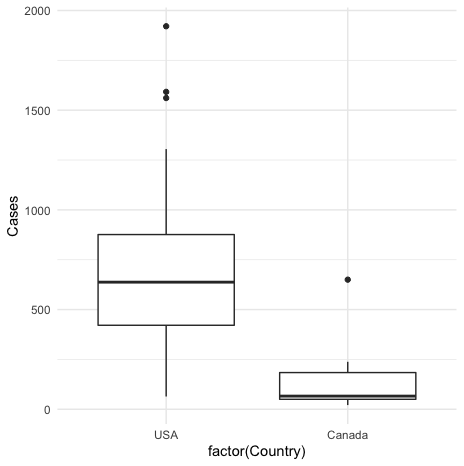
\includegraphics[width= 7cm]{ggplotcc.png}
  \captionof{figure}{cases by country}
  \label{fig:ggcc}
\end{figure}
Canada provinces and US states experienced similar drops in GDP:
\begin{figure}[H]
  \centering
  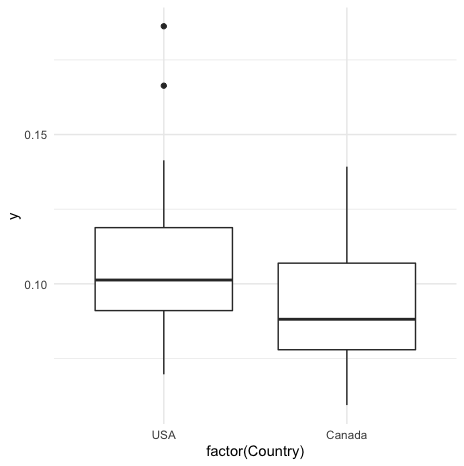
\includegraphics[width= 7cm]{ggplotgc.png}
  \captionof{figure}{GDP drop by country}
  \label{fig:gggc}
\end{figure}\\
\newpage
\subsubsection{Response variable vs covariates}
\noindent Scatter-plots of \textit{GDP drop} against each predictive variable:\\
Some outliers are present, and can potentially have high leverage in the multi-covariate model.
\begin{figure}[H]
\begin{minipage}{.5\textwidth}
  \centering
  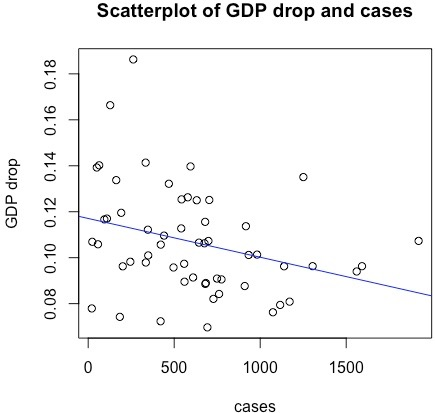
\includegraphics[width= 5.1cm]{cases.jpg}
  \captionof{figure}{Scatterplot of GDP drop vs cases}
  \label{fig:case}
\end{minipage}%
\begin{minipage}{.5\textwidth}
  \centering
  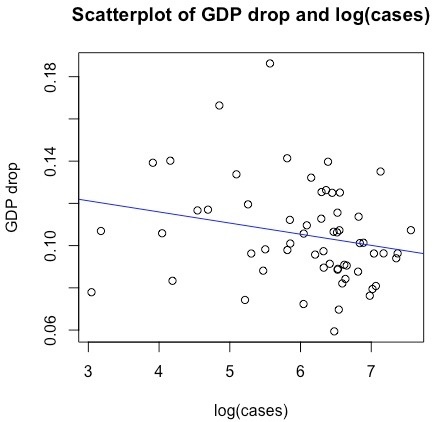
\includegraphics[width= 5.1cm]{cases2.jpg}
  \captionof{figure}{Scatterplot of GDP drop vs log(cases)}
  \label{fig:log(case)}
\end{minipage}%
\end{figure}
\begin{figure}[H]
\centering
\begin{minipage}{.5\textwidth}
  \centering
  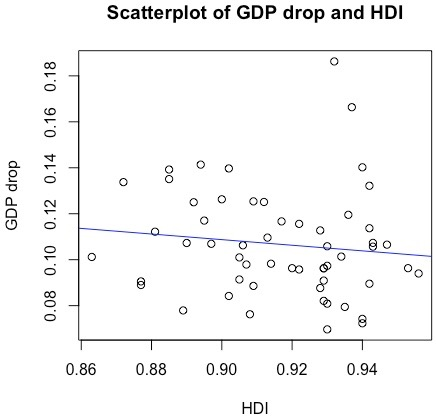
\includegraphics[width= 5.1cm]{HDI.jpg}
  \captionof{figure}{Scatterplot of GDP drop and HDI}
  \label{fig:HDI}
\end{minipage}%
\begin{minipage}{.5\textwidth}
  \centering
  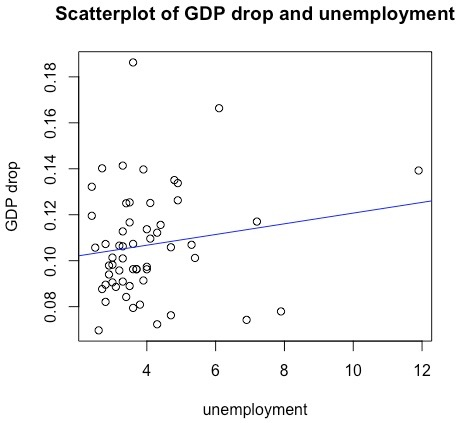
\includegraphics[width= 5.1cm]{unemployment.jpg}
  \captionof{figure}{Scatterplot of GDP drop and unemployment}
  \label{fig:unemploymeent}
\end{minipage}
\centering
\begin{minipage}{.5\textwidth}
  \centering
  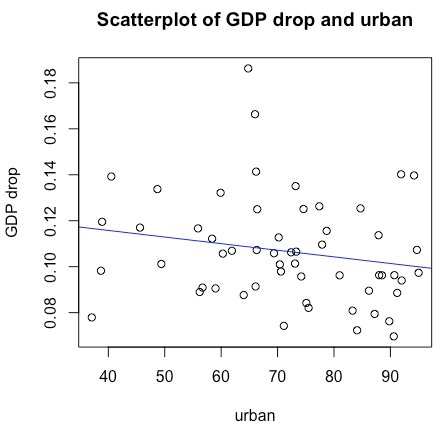
\includegraphics[width= 5.1cm]{urban.jpg}
  \captionof{figure}{Scatterplot of GDP drop and urban}
  \label{fig:urban}
\end{minipage}%
\begin{minipage}{.5\textwidth}
  \centering
  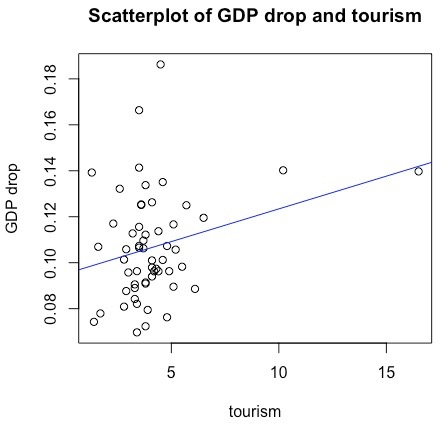
\includegraphics[width= 5.1cm]{tourism.jpg}
  \captionof{figure}{Scatterplot of GDP drop and tourism}
  \label{fig:tourism}
\end{minipage}
\end{figure}
\\
\noindent Furthermore, the correlation values between variables are calculated:
\begin{itemize}
    \item correlation between GDP drop and cases: -0.2593148
    \item correlation between GDP drop and urban:  -0.1690294
    \item correlation between GDP drop and tourism: 0.3113015
    \item correlation between GDP drop and unemployment: 0.09736781
    \item correlation between GDP drop and HDI: -0.1044564
\end{itemize}
As shown above, the correlation between the response variable and each covariate is quite moderate. \textit{Tourism} has the highest correlation with the response variable, at $0.3113015$.\\

\subsubsection{Correlation between covariates}
\noindent \textit{Cases}, \textit{urban} and \textit{HDI}
show relatively high correlation:
\begin{figure}[H]
  \centering
  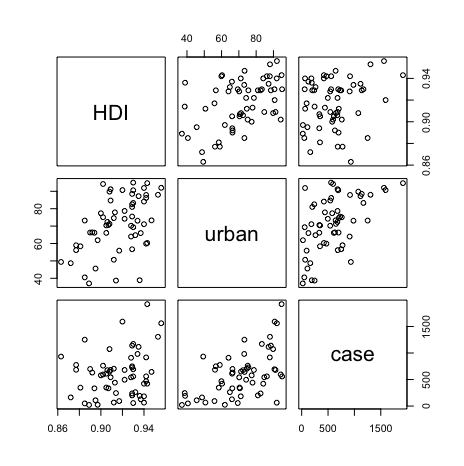
\includegraphics[width= 8cm]{correlation.png}
  \captionof{figure}{Matrix of scatter-plots}
  \label{fig:gggc}
\end{figure}

\subsection{Model Selection}
\subsubsection*{Full model}
\noindent We start with a model with all predictive variables:
\begin{verbatim}
mod.full <- lm(y~urban + tourism + case + HDI + unemploy + country)
\end{verbatim}
\begin{figure}[H]
\centering
  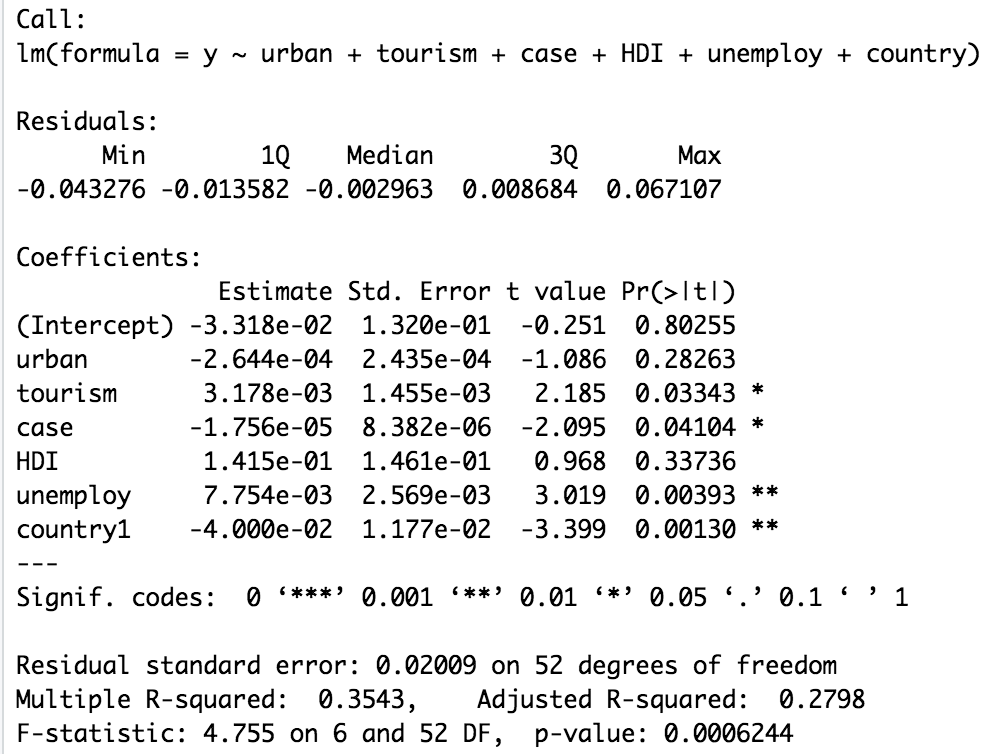
\includegraphics[width=8cm]{summary-full.png}
  \captionof{figure}{Summary for full model}
  \label{fig:summaryfull}
\end{figure}
\noindent The coefficients for \textit{case}, \textit{tourism}, \textit{unemployment} and \textit{country} are significant. \textit{Urban} and \textit{HDI} do not add much explanatory power in presence of \textit{cases}, which coincides with their relatively high correlation with \textit{cases}.

\subsubsection*{Alternative model}
\begin{verbatim}
mod.alt <- lm(y~urban + tourism + country)
\end{verbatim}
\begin{figure}[H]
\centering
  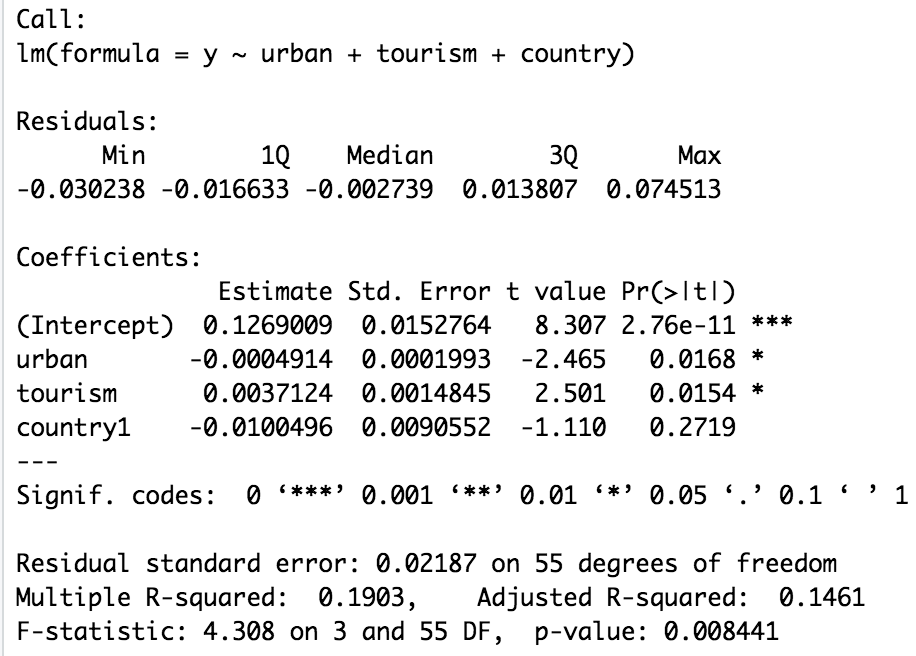
\includegraphics[width=8cm]{summary-alt.png}
  \captionof{figure}{Summary for alternative model}
  \label{fig:summaryalt}
\end{figure}
The \textbf{alternative model} doesn't include \textit{cases}. Although it indicates significance for \textit{urban}, it yields a lower $R^2$. There is not enough evidence to support the inclusion of \textit{urban}. 
\begin{verbatim}
mod.alt2 <- lm(y~HDI + tourism + country)
\end{verbatim} 
\begin{figure}[H]
\centering
  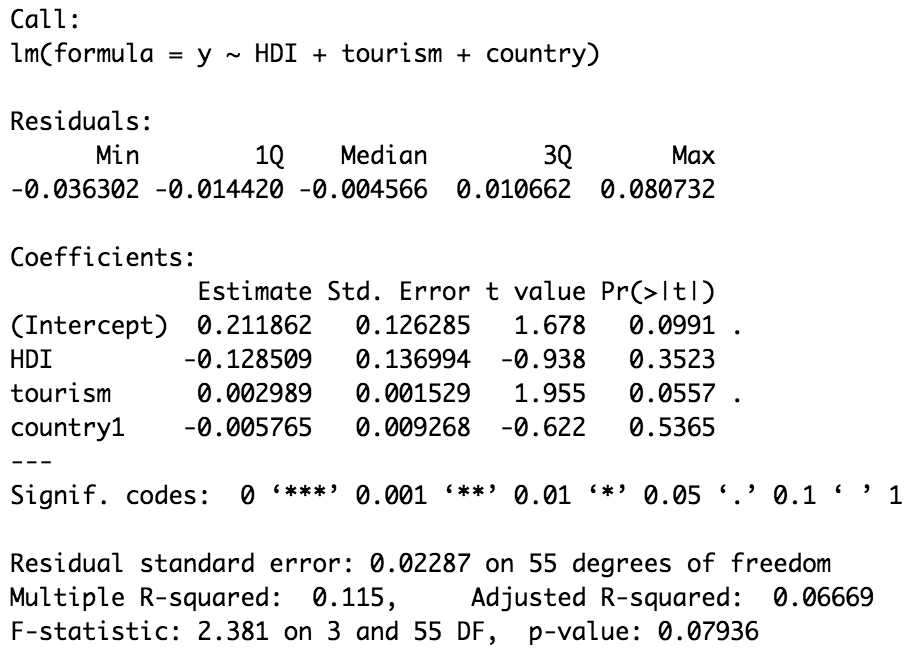
\includegraphics[width=8cm]{summary-alt2.png}
  \captionof{figure}{Summary for alt2 model}
  \label{fig:QQ}
\end{figure}
\textbf{Alt2 Model} also fails to show enough evidence to support the inclusion of \textit{HDI}. 
Results from \textbf{regsubset} from \textbf{leaps} confirms the findings above, and we have a \textbf{base model}:

\begin{verbatim}
mod.base <- lm(y~tourism + case + unemploy +country)
\end{verbatim}

\begin{figure}[H]
\centering
  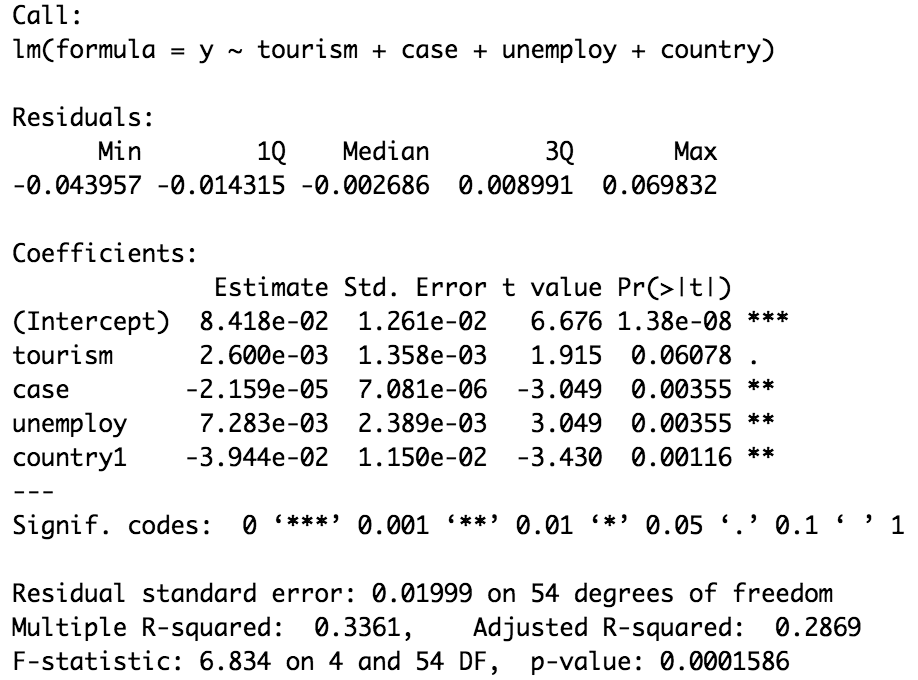
\includegraphics[width=8cm]{summary-base.png}
  \captionof{figure}{Summary for base model}
  \label{fig:QQ}
\end{figure}
 
\subsubsection*{Interaction model}
We further explore the possibility of including interaction terms. Given the difference in the social and economical structures between the two countries, and the discrepancies in how certain statistics are measured, it may be plausible to fit a model as below:
\begin{verbatim}
mod.interact <- lm(y~((tourism + case + unemploy) * country)
\end{verbatim}

\begin{figure}[H]
\centering
  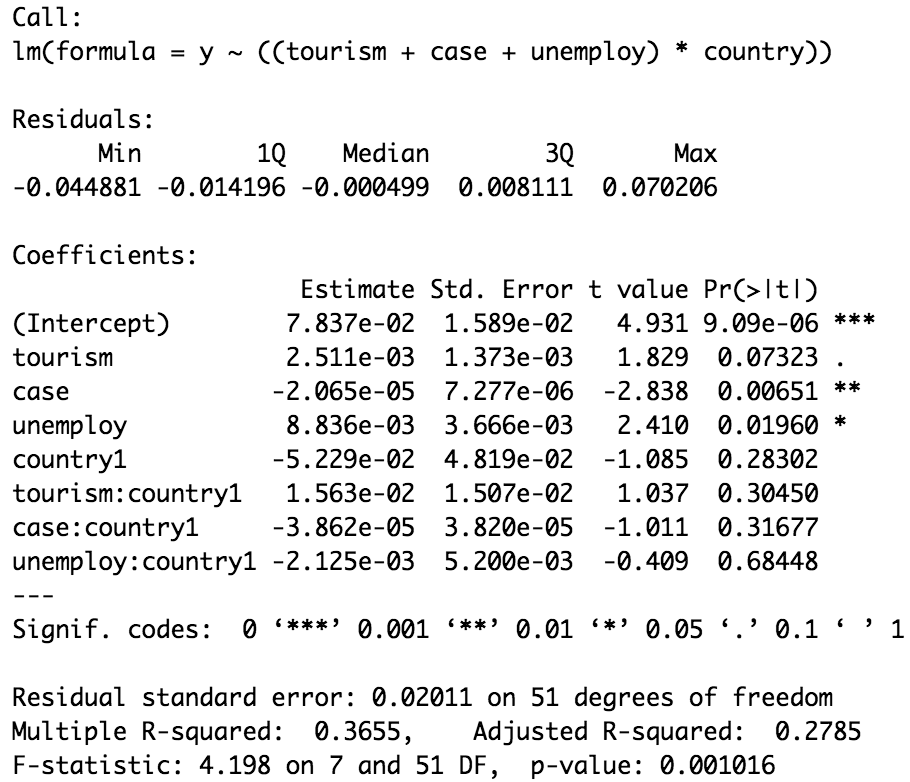
\includegraphics[width= 8cm]{summary-interact.png}
  \captionof{figure}{Summary for interaction model}
  \label{fig:QQ}
\end{figure}
 It yields a lower adjusted $R^2$ than the \textbf{base model}. Hence this is not adopted.
 
\subsubsection*{Log model}
Covid \textit{cases} tend to grow exponentially. We suspect $\log(case)$ could be a better measure of the severity of the pandemic.
\begin{verbatim}
mod.log <- lm(y~(tourism + log(case) + unemploy + country))
\end{verbatim}

\begin{figure}[H]
\centering
  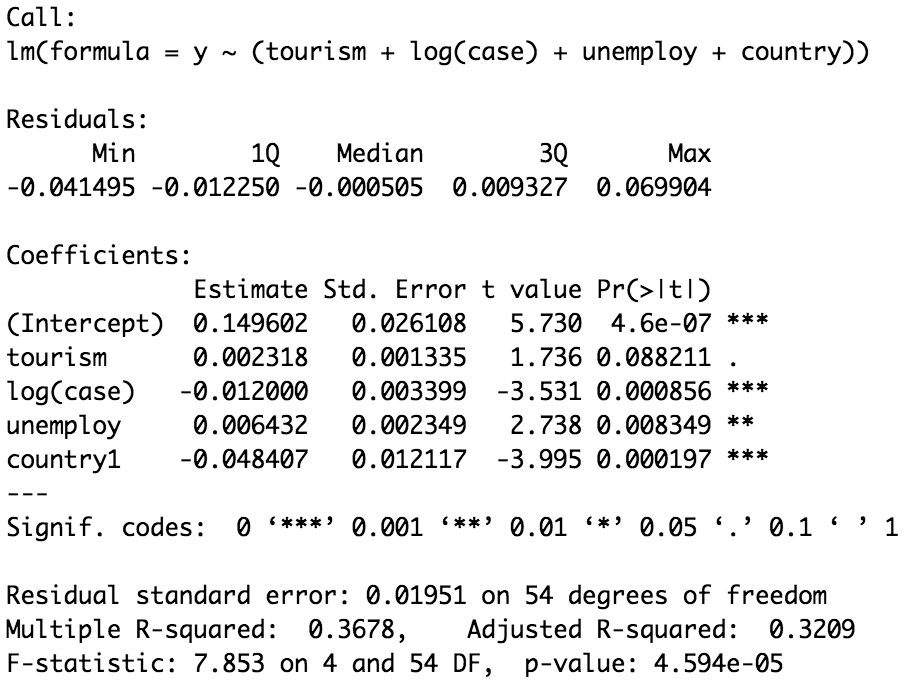
\includegraphics[width= 7.5cm]{summary-log.png}
  \captionof{figure}{Summary for log model}
  \label{fig:QQ}
\end{figure}\\

Compared to the \textbf{base model}, it yields a higher $R^2$.

Hence, the \textbf{log model} is selected:  \verb|lm(y~(tourism + log(case) + unemploy + country))|



\subsection{Diagnostic}
We examine the diagnostic plots of the selected model: \verb|lm(y~(tourism + log(case) + unemploy + country))|
\begin{figure}[H]
\centering
\begin{minipage}{.5\textwidth}
  \centering
  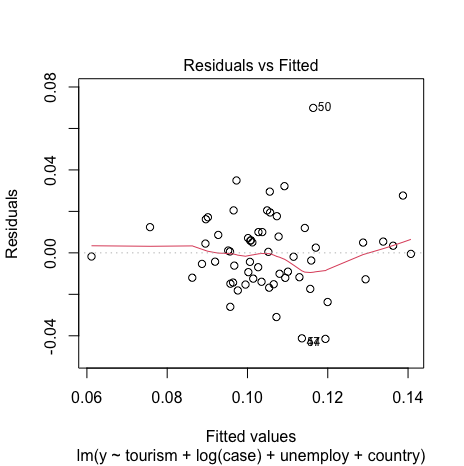
\includegraphics[width= 5.5cm]{residual.png}
  \captionof{figure}{Residual vs $\hat{y}$}
  \label{fig:resid}
\end{minipage}%
\begin{minipage}{.5\textwidth}
  \centering
  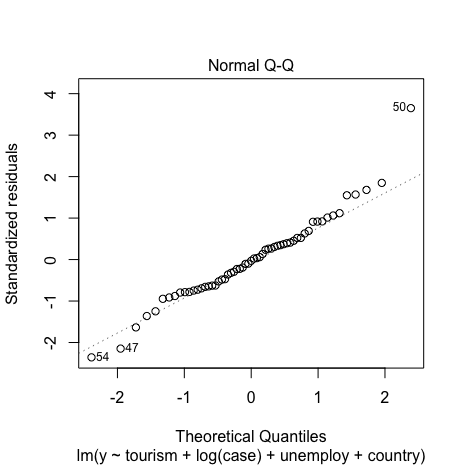
\includegraphics[width= 5.5cm]{qqplot.png}
  \captionof{figure}{QQ-plot for the selected model}
  \label{fig:QQ}
\end{minipage}
\end{figure}
The residual plot shows the points are roughly randomly scattered around the line of $y = 0$. The errors are mostly normally distributed with no obvious patterns.

The Q-Q plot falls around the dashed line, an indication that the assumption of normality of residuals is not violated. However, there exist a few residual values in the upper right of the plot are slightly higher than the estimated quantile values. 
 
We fit the residual plots of each individual variable to explore if polynomial terms are necessary to include:

\begin{figure}[H]
\centering
\begin{minipage}{.5\textwidth}
  \centering
  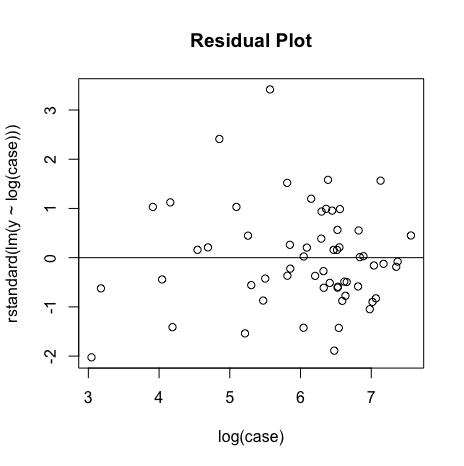
\includegraphics[width= 6cm]{logcase-res.png}
  \captionof{figure}{Residual vs log(cases)}
  \label{fig:resid-urban}
\end{minipage}%
\begin{minipage}{.5\textwidth}
  \centering
  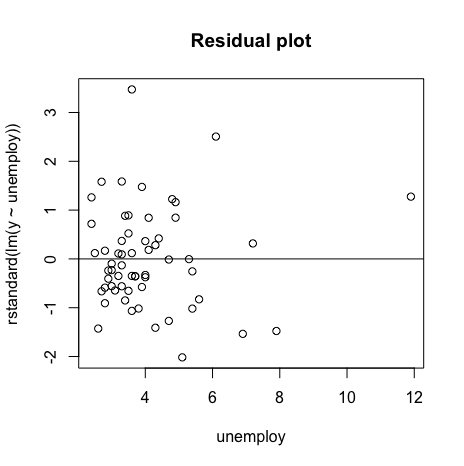
\includegraphics[width= 6cm]{unem-res.png}
  \captionof{figure}{Residual vs unemployment}
  \label{fig:resid-tour}
\end{minipage}
\end{figure}\\
\begin{figure}[H]
  \centering
  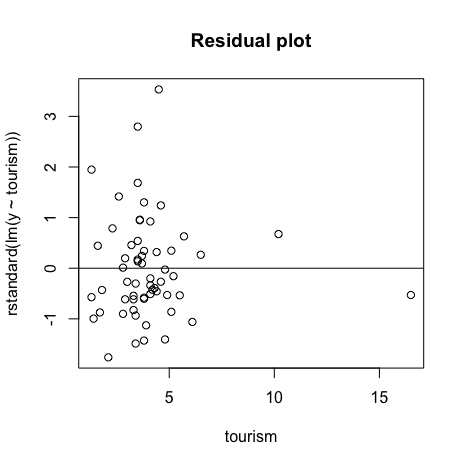
\includegraphics[width= 6cm]{tourism-res.png}
  \captionof{figure}{Residual vs tourism}
  \label{fig:resid-tour}
\end{figure}
We observe roughly symmetric distributions around $y = 0$ for all residual plots, and no obvious pattern is present. Thus, there is not enough evidence to include polynomial terms. However, we can see some outliers in x in certain graphs, so a leverage plot is created for further exploration:
\begin{figure}[H]
\centering
\begin{minipage}{.5\textwidth}
  \centering
  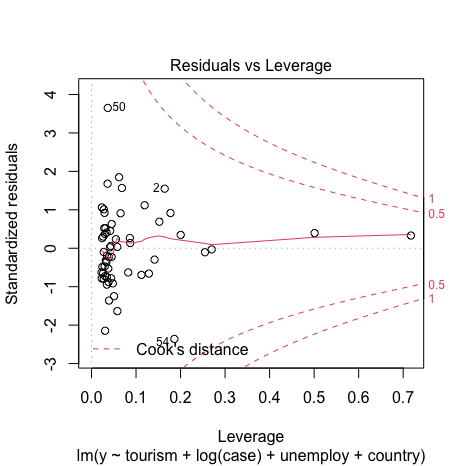
\includegraphics[width= 6.5cm]{leverage.png}
  \captionof{figure}{Leverage plot for the selected model}
  \label{fig:leverage}
\end{minipage}%
\end{figure}\\
All of the points have low to moderate leverage, given all the points lie within the 0.5 dashed line.

Diagnostic plots show no obvious fallacy in the chosen model. 

\newpage
\maketitle
\section{Conclusion} 

Statistics, including Tourism, log(Cases), Unemployment and the categorical variable, Country, were significant in explaining the decline in the output of the economy, measured by GDP. In contrast, HDI, an indicator of the development of the region prior to the outbreak, showed no important relationship with the extent of the economic impact. Urban population percentage does not contribute much explanatory power when Cases are included. 

States/Provinces that were suffering from inefficiency due to higher unemployment rates prior to the lock-downs were those who struggled from greater economic declines. States/Provinces with an economic structure that has high reliance on tourism also were more severely impacted. Moreover, states/provinces with less severe drop in economy are also the ones with more cases, which emphasizes the distinction between coping with the crisis from the public health standpoint and from the economic standpoint. Furthermore, the significance of the categorical variable, Country, acknowledges the differences in policies, economic structures, or even culture between these two countries, which can be further studied and discussed.

Finally, given the complex nature of this economic problem, a relatively low value of 0.36 for the $R^2$ is within our expectation. Nonetheless, we believe that including statistics that captures the broader economic fundamentals of a state/province may improve the $R^2$. For example, the percentage of GDP from the service sector can replace or use together with the percentage of GDP from Tourism. Other useful economic measurements may include median saving rate, an average measure for the digitization of companies and number of starting companies in 2019. 





\maketitle
\newpage
\section{Appendix \& Reference}\\
\noindent\textbf {4.1 Data Sources:}

\noindent \textbf{Change in GDP between Dec 31, 2019 to Jun 30, 2020:}\\
\textit{U.S. Department of Commerce}:\\
\url{https://www.bea.gov/sites/default/files/2020-10/qgdpstate1020_0.pdf}\\
\noindent \textbf{Covid-19 cases until June 30, 2020:}\\
\textit{CDC}:\\
\url{https://data.cdc.gov/Case-Surveillance/United-States-COVID-19-Cases-and-Deaths-by-State-o/9mfq-cb36/data}\\
\textit{CTV News}:\\ \url{https://www.ctvnews.ca/health/coronavirus/tracking-every-case-of-covid-19-in-canada-1.4852102}

\noindent \textbf{The number of cases per 100,000 people:}\\
\textit{New York Times}:
\url{https://www.nytimes.com/interactive/2020/us/coronavirus-us-cases.html}\\
\url{https://www.nytimes.com/interactive/2020/world/canada/canada-coronavirus-cases.html}

\noindent \textbf{Human Development Index:}\\
\textit{Global Data Lab}:
\url{https://globaldatalab.org/shdi/2018/indices/CAN+USA/?levels=4&interpolation=0&extrapolation=0&nearest_real=0}

\noindent \textbf{Unemployment rate:}\\
\textit{Statista}:
\url{https://www.statista.com/statistics/223675/state-unemployment-rate-in-the-us/}\\
\url{https://www.statista.com/statistics/442316/canada-unemployment-rate-by-provinces/}

\noindent \textbf{Tourism contribution:}\\
\textit{S&P Global}:
\url{https://www.spglobal.com/ratings/en/research/articles/200427-tourism-dependent-u-s-states-could-face-credit-pressure-from-covid-19-s-outsized-effects-on-the-industry-11457463}
\textit{Statistics Canada}:
\url{https://www150.statcan.gc.ca/n1/daily-quotidien/181010/t001b-eng.htm}

\noindent \textbf{Urban population Percentage:}\\
“Urban Percentage of the Population for States, Historical” by \textit{Iowa State University}:\\
\url{https://www.icip.iastate.edu/tables/population/urban-pct-states}\\
\textit{Statistic Canada}:
\url{https://www150.statcan.gc.ca/t1/tbl1/en/tv.action?pid=1710013501}\\

\newpage
\noindent\textbf{4.2 Data as CSV}\\
Data file: \url{https://docs.google.com/spreadsheets/d/1am06wfZij0vhpKDgi1kZnng2LpcY1DfYtATPkm9VSqw/edit?usp=sharing}
\end{document}
